%%%%%%%%%%%%%%%%%%%%%%%%%%%%%%%%% LAB-5 %%%%%%%%%%%%%%%%%%%%%%%%%%%%%%%%%%
%>>>>>>>>>>>>>>>>>>>>>>>>>> ПЕРЕМЕННЫЕ >>>>>>>>>>>>>>>>>>>>>>>>>>>>>>>>>>>
%>>>>> Информация о кафедре
%\newcommand{\year}{2021 г.}  % Год устанавливается автоматически
\newcommand{\city}{Санкт-Петербург}  %  Футер, нижний колонтитул на титульном листе
\newcommand{\university}{Национальный исследовательский университет ИТМО}  % первая строка
\newcommand{\department}{Факультет программной инженерии и компьютерной техники}  % Вторая строка
\newcommand{\major}{Направление программная инженерия}  % Треьтя строка
% Пусть будет. Проще закоментить лишнее.
\newcommand{\education}{Образовательная программа системное и прикладное программное обеспечение}  % четвертая строка
\newcommand{\specialization}{Специализация системное программное обеспечение}  % пятая строка

%<<<<< Информация о кафедре

%>>>>> Назание работы
\newcommand{\reporttype}{ОТЧЕТ ПО ДОМАШНЕЙ РАБОТЕ} % тип работы, (главный заголовок титульного листа)
\newcommand{\lab}{Лабораторная работа}          % вид работы
\newcommand{\labnumber}{№ 4}                    % порядковый номер работы
\newcommand{\subject}{Компьютерные сети}         % учебный предмет
\newcommand{\labtheme}{Работа с инструментом Wireshark \\и анализ сетевого трафика}            % Тема лабораторной работы

\newcommand{\student}{Тюрин Иван Николаевич}    % определение ФИО студента
\newcommand{\studygroup}{P33102}                 % определение учебной группы 
\newcommand{\teacher}{% принимающий
    Авксентьева Е. Ю.,\\[1mm]% ФИО лектора
    Алиев Т. И.% ФИО практика
}

%>>>>>>>>>>>>>>>>>>>>>> ПРЕАМБУЛА >>>>>>>>>>>>>>>>>>>>>>>>>

%>>>>>>>>>>>>>>>>>> ПРЕАМБУЛА >>>>>>>>>>>>>>>>>>>>
\documentclass[14pt,final,oneside]{extreport}% класс документа, характеристики
%>>>>> Разметка документа
\usepackage[a4paper, mag=1000, left=3cm, right=1.5cm, top=2cm, bottom=2cm, headsep=0.7cm, footskip=1cm]{geometry} % По ГОСТу: left>=3cm, right=1cm, top=2cm, bottom=2cm,
\linespread{1} % межстройчный интервал по ГОСТу := 1.5
%<<<<< Разметка документа

%>>>>> babel c языковым пакетом НЕ должны быть первым импортируемым пакетом
\usepackage[utf8]{inputenc}
\usepackage[T1,T2A]{fontenc}
\usepackage[russian]{babel}
%<<<<<

%\usepackage{cmap} %поиск в pdf

%>>>...>> прочие полезные пакеты
\usepackage{amsmath,amsthm,amssymb}
\usepackage{mathtext}
\usepackage{indentfirst}
\usepackage{graphicx}
\usepackage{float}
\graphicspath{{/home/ivan/itmo/informatics/latex}}
\DeclareGraphicsExtensions{.pdf,.png,.jpg}
%\usepackage{bookmark}

\usepackage[dvipsnames]{xcolor}
\usepackage{hyperref}  % Использование ссылок
\hypersetup{%  % Настройка разметки ссылок
    colorlinks=true,
    linkcolor=blue,
    filecolor=magenta,      
    urlcolor=magenta,
    %pdftitle={Overleaf Example},
    %pdfpagemode=FullScreen,
}

\usepackage{diagbox}
\usepackage[letterspace=150]{microtype} % Спэйсинг (межбуквенный интервал для саголовка) \lsstyle
% \usepackage{csvsimple} %импорт содержимого таблицы из csv

%>>> верстка в 2 колонки
\usepackage{multicol} % многоколоночная верстка
\setlength{\columnsep}{.15\textwidth} % определение ширины разделителя между колонками

\usepackage{tikz} % пакет для векторной графики, чтобы рисовать красивый разделитель колонок
% %> кастомный разделитель колонок
% \usetikzlibrary{arrows.meta,decorations.pathmorphing,backgrounds,positioning,fit,petri}
% \usepackage{multicolrule} % Для кастомизации разделителя колонок
% \SetMCRule{                     % кастомизация разделителя колонок multicolrule
%     width=2pt,
%     custom-line={               % Tikz код для кастомизации линии разделителя
%         \draw [                 % Рисовать
%             decorate,           % декорированную (требуются спец настройки пакетов tikz (см. импорт выше)
%             decoration={        % вид декорирования
%                 snake, % Тип - змейка (волнистая)
%                 amplitude=.5mm, % ширина волн
%                 pre length=0mm, % участок прямой линии от начала
%                 %segment length=0mm, % учасок волнистой линии
%                 post length=0mm % участок прямой линии от конца
%             },
%             line width=1pt,
%             step=10pt
%         ] 
%         (TOP) to (BOT); % сверху и до низа колонки
%     }, 
%     extend-top=-5pt, % Вылезти за верхнюю границу колонки 
%     extend-bot=-7pt % Вылезти за нижнюю границу колонки  
% }
%% < кастомный разделитель колонок
%%<<< верстка в 2 колонки

%>>>>> Использование листингов
\usepackage{listings} 
\usepackage{caption}
\DeclareCaptionFont{white}{\color{white}} 
\DeclareCaptionFormat{listing}{\colorbox{gray}{\parbox{\textwidth}{#1#2#3}}}

\captionsetup[lstlisting]{format=listing,labelfont=white,textfont=white} % Настройка вида описаний
\lstset{  % Настройки вида листинга
inputencoding=utf8, extendedchars=\true, keepspaces = true, % поддержка кириллицы и пробелов в комментариях
language={},            % выбор языка для подсветки (здесь это Pascal)
basicstyle=\small\sffamily, % размер и начертание шрифта для подсветки кода
numbers=left,               % где поставить нумерацию строк (слева\справа)
numberstyle=\tiny,          % размер шрифта для номеров строк
stepnumber=1,               % размер шага между двумя номерами строк
numbersep=5pt,              % как далеко отстоят номера строк от подсвечиваемого кода
backgroundcolor=\color{white}, % цвет фона подсветки - используем \usepackage{color}
showspaces=false,           % показывать или нет пробелы специальными отступами
showstringspaces=false,     % показывать илигнет пробелы в строках
showtabs=false,             % показывать или нет табуляцию в строках
frame=single,               % рисовать рамку вокруг кода
tabsize=2,                  % размер табуляции по умолчанию равен 2 пробелам
captionpos=t,               % позиция заголовка вверху [t] или внизу [b] 
breaklines=true,            % автоматически переносить строки (да\нет)
breakatwhitespace=false,    % переносить строки только если есть пробел
escapeinside={\%*}{*)}      % если нужно добавить комментарии в коде
}

\definecolor{codegreen}{rgb}{0,0.6,0}
\definecolor{codegray}{rgb}{0.5,0.5,0.5}
\definecolor{codepurple}{rgb}{0.58,0,0.82}
\definecolor{backcolour}{rgb}{0.95,0.95,0.92}

\lstdefinestyle{mystyle}{
    backgroundcolor=\color{backcolour},   
    commentstyle=\color{codegreen},
    keywordstyle=\color{magenta},
    numberstyle=\tiny\color{codegray},
    stringstyle=\color{codepurple},
    basicstyle=\ttfamily\footnotesize,
    breakatwhitespace=false,         
    breaklines=true,                 
    captionpos=b,                    
    keepspaces=true,                 
    numbers=left,                    
    numbersep=5pt,                  
    showspaces=false,                
    showstringspaces=false,
    showtabs=false,                  
    tabsize=2
}
\lstset{style=mystyle}
%<<<<< Использование листингов


\sloppy % Решение проблем с переносами (с. 119 книга Львовского)
\emergencystretch=25pt


%>>>>>>>>>>>>>>>> ДОПОЛНИТЕЛЬНЫЕ КОМАНДЫ {Для соответствия ГОСТ} >>>>>>>>>>>>>>
%>>>>>> математические функции для удобства
\newcommand{\tx}{\text}
\newcommand{\eps}{\varepsilon}
\renewcommand{\phi}{\varphi}
\newcommand{\limit}{\displaystyle\lim}
\newcommand{\oo}{\infty}
\newcommand{\De}{\Delta}
\newcommand{\cd}{\cdot}
\newcommand{\df}{\partial}
\newcommand{\ndash}{\textendash}
\newcommand{\mdash}{\textemdash}

%>>>>> Аннотирование
\newcommand{\note}[2]{\overbrace{#1}^{#2}}% скобка сверху для комментария
% \overset{}{}% для указания символа над другим смиволом
% \underset{}{}% для указания символа под другим смиволом
%<<<<< Аннотирование

%>>>>>> Матрицы
\DeclareMathOperator{\rank}{rank}
\newcommand{\tvec}[1]{\mathbfit{#1}}% "text vector"
\newcommand{\mtx}[1]{\mathrm{#1}}
\newcommand{\transposed}[1]{{#1}^{\mathrm{T}}}
%>>>>>> Матрицы

%>>>>> Скобки
\newcommand{\lt}{\left}
\newcommand{\rt}{\right}
\newcommand{\la}{\langle}% '<'
\newcommand{\ra}{\rangle}% '>'
\newcommand{\avg}[1]{\langle{#1}\rangle}% '<X>'
%<<<<< Скобки

%>>>>> Дроби
\newcommand{\cf}[2]{\cfrac{#1}{#2}}
\newcommand{\fr}[2]{\frac{#1}{#2}}
%<<<<< Дроби


%>>>>> Стрелки
\newcommand{\Rarr}{\Rightarrow}% ⇒ следствие | лучше использовать \implies
\newcommand{\LRarr}{\Leftrightarrow}% равносильно | лучше  использовать \iff
\newcommand{\rarr}{\xrightarrow{}}% → стрелка вправо
\newcommand{\nwarr}{\nwarrow}% ↖ север-запад стрелка
\newcommand{\nearr}{\nearrow}% ↗ север-восток стрелка
\newcommand{\swarr}{\swarrow}% ↙ юг-запад стрелка
\newcommand{\searr}{\searrow}% ↘ юг-восток стрелка

\newcommand{\raises}{\nwarrow}% возрастает
\newcommand{\increases}{\nwarrow}% возрастает
\newcommand{\falls}{\swarrow}% убывает
\newcommand{\decreases}{\swarrow}% убывает

%{{{
\makeatletter
\newcommand{\impliesby}[2][]{\ext@arrow 0359\Leftrightarrowfill@{#1}{#2}}% следствие с надписью
\makeatother
%}}}

%{{{
\makeatletter
\newcommand{\iffby}[2][]{\ext@arrow 0359\Rightarrowfill@{#1}{#2}}% равносильность с надписью
\makeatother
%}}}
%<<<<< Стрелки

% Функции для удобного описания формул: https://tex.stackexchange.com/questions/95838/how-to-write-a-perfect-equation-parameters-description



%<<<<<< математические функции для удобства
%>>>>>> Стиль текста
\newcommand{\hex}[1]{\texttt{0{\footnotesize{x}}#1}}
\newcommand{\ttt}[1]{\texttt{#1}}
%<<<<<< Стиль текста

\newcommand\Chapter[3]{%
    % Принимает 3 аргумента - название главы и дополнительный заголовок и множитель ширины загловка (можно ничего)
    \refstepcounter{chapter}%
    \chapter*{%
        %\hfill % заполнение отступом пространства до заголовка
        \begin{minipage}{#3\textwidth} % Можно изменить ширину министраницы (заголовка)
            \flushleft % Выранивание заголовка по левому краю параграфа (заголовка)
            %\flushright % Выранивание заголовка по правому краю параграфа (заголовка)
            \begin{huge}%
                % Отключена нумерация глав в тексте:
                % \textbf{\chaptername\ \arabic{chapter}\\}
                \textbf{#1}% Первый заголовок
            \end{huge}%
            \\% Перенос сторки
            \begin{Huge}
                #2% Второй заголовок
            \end{Huge}
        \end{minipage}
    }%
    % Отключена нумерация для chapter в toc (table of contents), т.е. Оглавлении (Содержании):
    % \addcontentsline{toc}{chapter}{\arabic{chapter}. #1}
    % Представление главы в содержании:
    \addcontentsline{toc}{chapter}{#1. #2}%
}

\newcommand\Section[1]{
    % Принимает 1 аргумент - название секции
    \refstepcounter{section}
    \section*{%
        \raggedright
        % Отключена дополнительная нумерация chapter в section в тексте документа:
        % \arabic{chapter}.\arabic{section}. #1}
        % Отключена любая нумарация section в тексте документа: 
        \arabic{section}. #1%
    }
    
    % Отключена дополнительная нумерация chapter в section в toc (table of contents) Оглавлении (Содержании):
    % \addcontentsline{toc}{section}{\arabic{chapter}.\arabic{section}. #1}
    \addcontentsline{toc}{section}{\arabic{section}. #1} 
}


\newcommand\Subsection[1]{
    % Принимает 1 аргумент - название подсекции
    \refstepcounter{subsection}
    \subsection*{%
        \raggedright%
        % Отключена дополнительная нумерация chapter в section в тексте документа (можно добавить отступ с помощью \hspace*{12pt}):
        % \arabic{chapter}.\arabic{section}.\arabic{subsection}. #1}
        \arabic{section}. \arabic{subsection}. #1
    }
    % Отключена дополнительная нумерация chapter в section в Оглавлении (Содержании):
    %\addcontentsline{toc}{subsection}{\arabic{chapter}.\arabic{section}.\arabic{subsection}. #1}
    \addcontentsline{toc}{subsection}{\arabic{subsection}. #1}
}


\newcommand\Figure[4]{
    % Принимает 4 аргумента - название файла изображения, ее размер в тексте, описание, лэйбл (псевдоним в формате "fig:name") 
    %
    \refstepcounter{figure}
    \begin{figure}[H] %- \usepackage {float} %[h]
        \begin{center}
            \fbox{
                \includegraphics[width=#2]{#1}
            }
        \end{center}
        \begin{center}
            Рис.~\arabic{figure}. #3.
        \end{center}
        %\caption{#3}
        \label{fig:#4}
    \end{figure}
}


\newcommand\Table[3]{
    % Принимает 3 аргумента --- лэйбл name(#1) (псевдоним в формате "tab:name"), ее описание(#2), содержание таблицы(#3)
    % ВАЖНО!: от этого способа страдает нумерация описаний, можно использовать создание таблиц через googlesheet
    %
    \renewcommand{\arraystretch}{1.2} % Установка высоты строки таблицы по умолчанию, увеличенное на 0.2 пункта
    % \refstepcounter{table}% увеличение счетчика таблиц
    \begin{table}[Htpb]% "right Here", "top", "new page", "bottom"
        \label{tab:#1}% лэйбл таблицы, для ссылок
        \resizebox{\columnwidth}{!}{% сжимает очень широкие таблицы, чтобы вместить на страницу
             #3% Содержимое таблицы
        }
        % 
        \caption{#2}% Описание стандартными средствами для используемого окружения (table)
        % \captionof{table}{#2}% Описание стандартными средствами
        % \captionof*{figure}{\flushleft \textsc\textbf{Рис. 1.}}% Описание стандартными средствами, как рисунка
        %
        %%> кастомное описание
        % \begin{flushleft}% Кастомное описание
        %     % \textsf{%
        %         \textbf{%
        %             \\[2mm]
        %             #2% Описание к картинке
        %         }%
        %         % \\[8mm]% Отступ
        %     % }%
        % \end{flushleft}
        %%< кастомное описание
    \end{table}
    \renewcommand{\arraystretch}{1} % возврат установка высоты строки таблицы по умолчанию на 1
}


\newcommand\CustomFigure[4]{ % multicols не умеют в table и figure, поэтому приходится извращаться % вставка таблицы с меткой рисунка
    % Принимает 4 аргумента - название файла изображения, ее размер в тексте, описание, лэйбл (псевдоним в формате "fig:name") 
    %
    \refstepcounter{figure}
    \begin{figure}[ht]% "here", "top"
        \begin{center}
            \includegraphics[width=#2]{#1}
        \end{center}
        %
        %\caption{#3}
        \captionof{figure}{#3}% описание стандартными средствами
        % \begin{center}
        \begin{flushleft} % Кастомное описание
            \textbf{%
                #3% Текст описания
            }
        \end{flushleft}
        % \end{center}
        %
        \label{fig:#4}% Лэйбл, для ссылок
    \end{figure}
}


\newcommand\CustomTableFigure[3]{% multicols не умеют в table и figure, поэтому приходится извращаться % вставка таблицы с меткой рисунка
    %
    % Принимает 3 аргумента --- лэйбл name(#1) (псевдоним в формате "tab:name"), ее описание(#2), содержание таблицы(#3) 
    %
    \begin{center}
        \refstepcounter{figure}
        \label{tab:#1}% лэйбл таблицы, для ссылок
        \resizebox{\columnwidth}{!}{% сжимает очень широкие таблицы, чтобы вместить на страницу
            #3% Содержание таблицы
        }
        % 
        \captionof{figure}{#2}% Описание стандартными средствами
        % \captionof*{figure}{\flushleft \textsc\textbf{Рис. 1.}}% Описание стандартными средствами
        %
        \begin{flushleft}% Кастомное описание
            % \textsf{%
                \textbf{%
                    \\[2mm]
                    #2% Описание к картинке
                }%
                % \\[8mm]% Отступ
            % }%
        \end{flushleft}
    \end{center}
}


\newcommand{\InkscapeFigure}[4]{% Вставки иллюстраций из Inkscape (pdf+latex)
    %
    % Принимает 4 параметра: #1 название файла, #2 описание, #3 лейбл #4 размер
    %
    % \begin{minipage}{#4}
        \begin{figure}[htbp]
            \centering
            \def\svgwidth{#4}
            \import{./figures/}{#1.pdf_tex}
            \caption{#2}
            \label{fig:#3}
        \end{figure}
    % \end{minipage}
}


\newcommand\Equation[3]{% Кастомное оформление выражений
    %
    % Принимает 3 аргумента --- лэйбл name (#1) (псевдоним в формате "tab:name"), его описание(#2), содержание выражения (#3) 
    %
    \textbf{#2}% описание
    \begin{equation}
        #3% содержимое выражений
        \label{eq:#1}% лэйбл
    \end{equation}
}

%<<<<<<<<<<<<<<<<<<<<<<<<<<<< ДОПОЛНИТЕЛЬНЫЕ КОМАНДЫ <<<<<<<<<<<<<<<<<<<<<<<<<<

%<<<<<<<<<<<<<<<<<<<<<< ПРЕАМБУЛА <<<<<<<<<<<<<<<<<<<<<<<<<



%%%%%%%%%%%%%%%%%%% СОДЕРЖИМОЕ ОТЧЕТА %%%%%%%%%%%%%%%%%%%%%
%>>>>>>>>>>>>>>> ''''''''''''''''''''''' >>>>>>>>>>>>>>>>>>
\begin{document}


%>>>>>>>>>>>>>>>> ОПРЕДЕЛЕНИЕ НАЗВАНИЙ >>>>>>>>>>>>>>>>>>>>
% Переоформление некоторых стандартных названий
%\renewcommand{\chaptername}{Лабораторная работа}
\renewcommand{\chaptername}{\lab\ \labnumber} % переименование глав
\def\contentsname{Содержание} % переименование оглавления
%<<<<<<<<<<<<<<<< ОПРЕДЕЛЕНИЕ НАЗВАНИЙ <<<<<<<<<<<<<<<<<<<<
% \setlength{\itemsep}{0pt} % установка расстояния между строчками в списках можно использовать локально внутри списка списке
% \setlength{\parskip}{0pt} % 
% \setlength{\parsep}{0pt}  % 

%>>>>>>>>>>>>>>>>> ТИТУЛЬНАЯ СТРАНИЦА >>>>>>>>>>>>>>>>>>>>>
%>>>>>>>>>>>>>>>>>>> ТИТУЛЬНЫЙ ЛИСТ >>>>>>>>>>>>>>>>>>>>>>>
\begin{titlepage}

    % Название университета
    \begin{center}
    \textsc{%
        \university\\[5mm]
        \department\\[2mm]
        \major\\
        \education\\
        \specialization\\
    }

    \vfill
    % Название работы
    \textbf{\reporttype\ \labnumber\\[3mm]
    курса <<\subject>> \\[6mm]
    по теме: <<\labtheme>>\\[3mm]
    }
    \end{center}


\vfill
\hfill
% Информация об авторе работы и проверяющем
\begin{minipage}{.5\textwidth}
    \begin{flushright}
        
            
        Выполнил студент:\\[2mm] 
        \student\\[2mm]
        группа: \studygroup\\[5mm]

        Преподаватель:\\[2mm] 
        \teacher

    \end{flushright}
\end{minipage}

\vfill

    % Нижний колонтитул первой страницы
    \begin{center}
        \city, \the\year\,г.
    \end{center}

\end{titlepage}
%<<<<<<<<<<<<<<<<<<< ТИТУЛЬНЫЙ ЛИСТ <<<<<<<<<<<<<<<<<<<<<<<


%<<<<<<<<<<<<<<<<< ТИТУЛЬНАЯ СТРАНИЦА <<<<<<<<<<<<<<<<<<<<<


%>>>>>>>>>>>>>>>>>>>>> СОДЕРЖАНИЕ >>>>>>>>>>>>>>>>>>>>>>>>>
% Содержание
\tableofcontents
%<<<<<<<<<<<<<<<<<<<<< СОДЕРЖАНИЕ <<<<<<<<<<<<<<<<<<<<<<<<<


%%%%%%%%%%%%%%%%%%%%%%% КОД РАБОТЫ %%%%%%%%%%%%%%%%%%%%%%%%
%>>>>>>>>>>>>>>>>>>>'''''''''''''''''>>>>>>>>>>>>>>>>>>>>>
\newpage
\Chapter{\lab\ \labnumber}{\labtheme}{}

\Section{Цель работы}

Цель работы – изучить структуру протокольных блоков данных, 
анализируя реальный трафик на компьютере студента с помощью бесплатно 
распространяемой утилиты Wireshark.

В процессе выполнения домашнего задания выполняются наблюдения за 
передаваемым трафиком с компьютера пользователя в Интернет и в обратном 
направлении. Применение специализированной утилиты Wireshark позволяет 
наблюдать структуру передаваемых кадров, пакетов и сегментов данных 
различных сетевых протоколов. При выполнении УИР рекомендуется выполнить 
анализ последовательности команд и определить назначение служебных данных, 
используемых для организации обмена данными в протоколах: ARP, DNS, FTP, 
HTTP, DHCP.

\textbf{Задание}
\begin{enumerate}
    \item Запустить Wireshark (иногда для этого требуются права 
Администратора). В появившемся окне выбрать интерфейс, для которого 
необходимо осуществлять анализ проходящих через него пакетов. В 
качестве интерфейса, используемого для захвата трафика, выбрать 
физический адаптер, через который компьютер подключён к Интернету 
(обычно этот адаптер называется Local или «Подключение по локальной 
сети»). Если меню для выбора адаптера не появляется при запуске 
Wireshark, нужно запустить из «Меню» команду «Capture->Options».
После выбора адаптера, нужно запустить процесс захвата трафика 
(кнопка Start).
\item Инициировать процесс передачи трафика по сети (например, в браузере 
открыть сайт, заданный по варианту, или запустить соответствующую 
сетевую утилиту – см. ниже).
\item Установить значение «Фильтра», чтобы из всего множества 
перехватываемых пакетов Wireshark отобразил только те, которые имеют 
отношение к выполняемому заданию. Для корректного создания фильтра 
следует пользоваться всплывающими подсказками Wireshark, которые 
активизируются при наборе фильтра. В качестве альтернативного 
способа можно использовать интерактивный конструктор фильтра, 
нажав на кнопку «Expression» в правой части элемента «Фильтр».
\item Дождаться появления данных в списке захваченных пакетов и убедиться, 
что количество пакетов достаточно для выполнения задания.
\item  Сохранить захваченный трафик в файл-трассу (pcap). Указанный файл 
нужно предъявить по первому требованию преподавателя во время 
защиты, если в этом возникнет необходимость.
\item  Описать в отчёте структуру наблюдаемых PDU (кадров, пакетов, 
сегментов) как для запросов, так и ответов. Указать название и 
назначение всех заголовков всех уровней OSI-модели в пакетах с учётом 
порядка инкапсуляции (для этого нужно раскрывать соответствующие 
значки «+» в поле с детальной информацией о выбранном пакете).
\item  Написать в отчёте ответы на вопросы задания (для этого может 
потребоваться самостоятельно изучить назначение соответствующей 
заданию сетевой утилиты, использованной для создания трафика).
\item  Поместить в отчёт скриншоты окна Wireshark, иллюстрирующие ответы 
из вышеуказанных п.6 и п.7.
\end{enumerate}

Адрес сайта, в котором по очереди встречаются инициалы (ФИО) 
студента в латинской транскрипции:

\begin{align*}
    \text{Тюрин Иван Николаевич} \to\text{tin}  \to  \text{tinkoff.ru}
\end{align*}

Найдем нужный IP-адрес с помощью команды \verb|nslookup tinkoff.ru|.

Получаем IPv4 адрес \verb|178.248.236.218|.

Для Wireshark используем маску \verb|ip.addr == 178.248.236.218|\;.

\newpage
\Section{Выполнение задания}

\Subsection{Анализ трафика утилиты ping}

Команды для выполнения: \verb|ping -l 100 tinkoff.ru|\;.

Shell с командой ping: \ref{fig:ping-shell}; результат захвата трафика в Wireshark: \ref{fig:ping-wireshark}.

\begin{figure}[h]
    \centering
    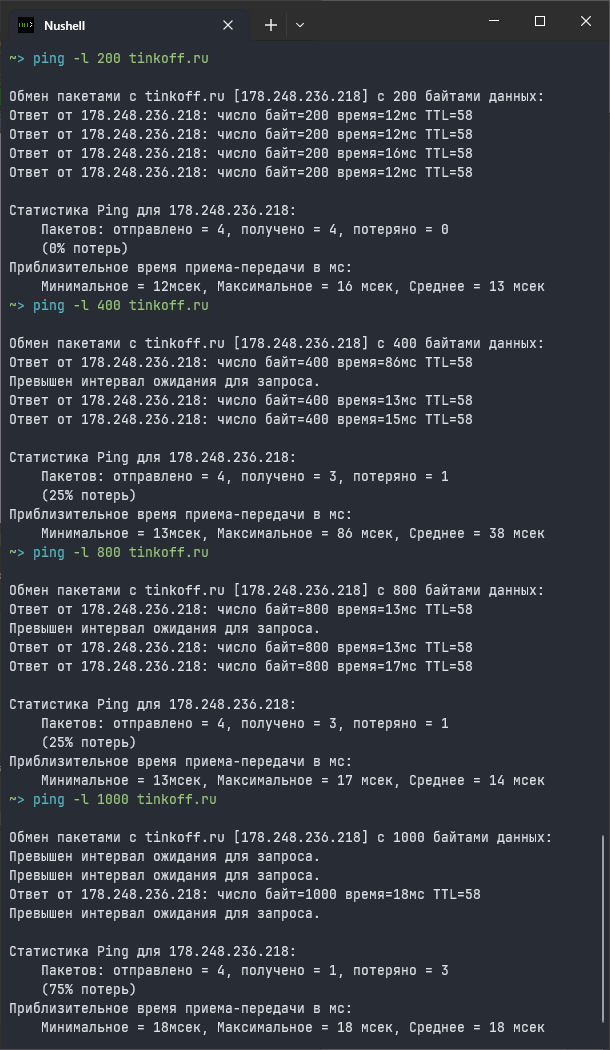
\includegraphics[width=0.8\linewidth]{res/ping-shell.png}
    \caption{Enter Caption}
    \label{fig:ping-shell}
\end{figure}

\begin{figure}[h]
    \centering
    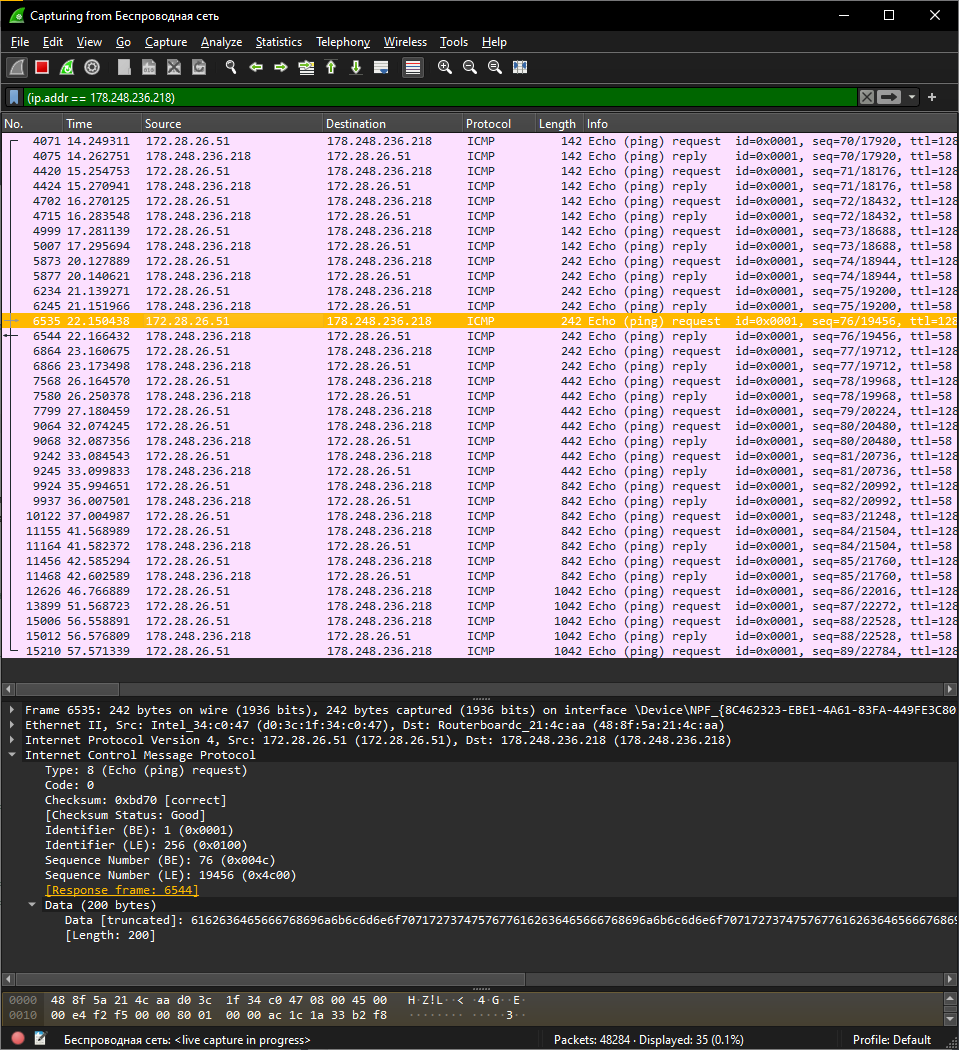
\includegraphics[width=1\linewidth]{res/ping-wireshark.png}
    \caption{Ping в Wireshark}
    \label{fig:ping-wireshark}
\end{figure}

\begin{enumerate}
    \item Имеет ли место фрагментация исходного пакета, какое поле на это 
указывает? --- Да, при больших пакетах, появились фрагменты Fragmented IP protocol
    \item Какая информация указывает, является ли фрагмент пакета последним 
или промежуточным? --- Флаг MF = 0.
        \begin{figure}[H]
            \centering
            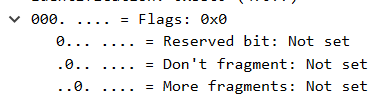
\includegraphics[width=0.5\linewidth]{res/ping-mf.png}
            \caption{ping MF}
            \label{fig:ping-mf}
        \end{figure}
    \item Чему равно количество фрагментов при передаче ping-пакетов? --- 3)	Количество фрагментов при передаче ping-пакетов может изменяться в зависимости от размера пакета и максимального размера передаваемых данных
    \item Построить график, в котором на оси абсцисс находится размер\_пакета, а 
по оси ординат – количество фрагментов, на которое был разделён 
каждый ping-пакет.
        \begin{figure}[H]
            \centering
            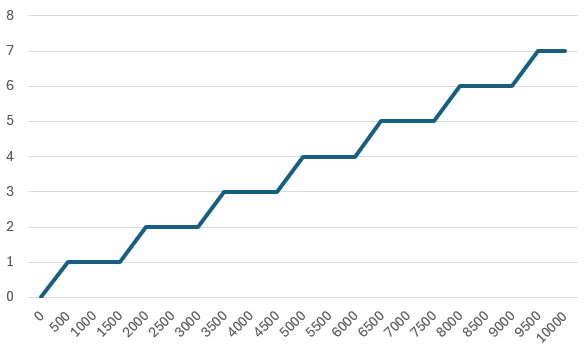
\includegraphics[width=0.75\linewidth]{res/ping-fragmentation.png}
            \caption{Фрагментация ping-пакетов}
            \label{fig:ping-fragmantation}
        \end{figure}
    \item Как изменить поле TTL с помощью утилиты ping? --- Добавить ключ -i
    \item Что содержится в поле данных ping-пакета? --- Символы английского алфавита
\end{enumerate}

\Subsection{ Анализ трафика утилиты tracert (traceroute)}

Команда для выполнения: \verb|tracert -d tinkoff.ru|\;.

Терминал с командой \verb|tracert|: \ref{fig:tracert-shell}; результат захвата трафика в Wireshark: \ref{fig:tracert-wireshark}.

\begin{figure}[h]
    \centering
    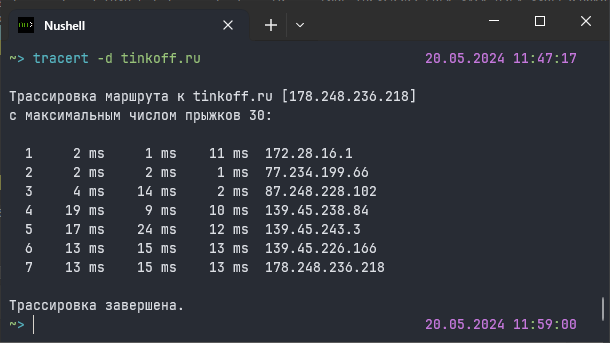
\includegraphics[width=1\linewidth]{res/tracert-shell.png}
    \caption{Tracert в консоли}
    \label{fig:tracert-shell}
\end{figure}

\begin{figure}
    \centering
    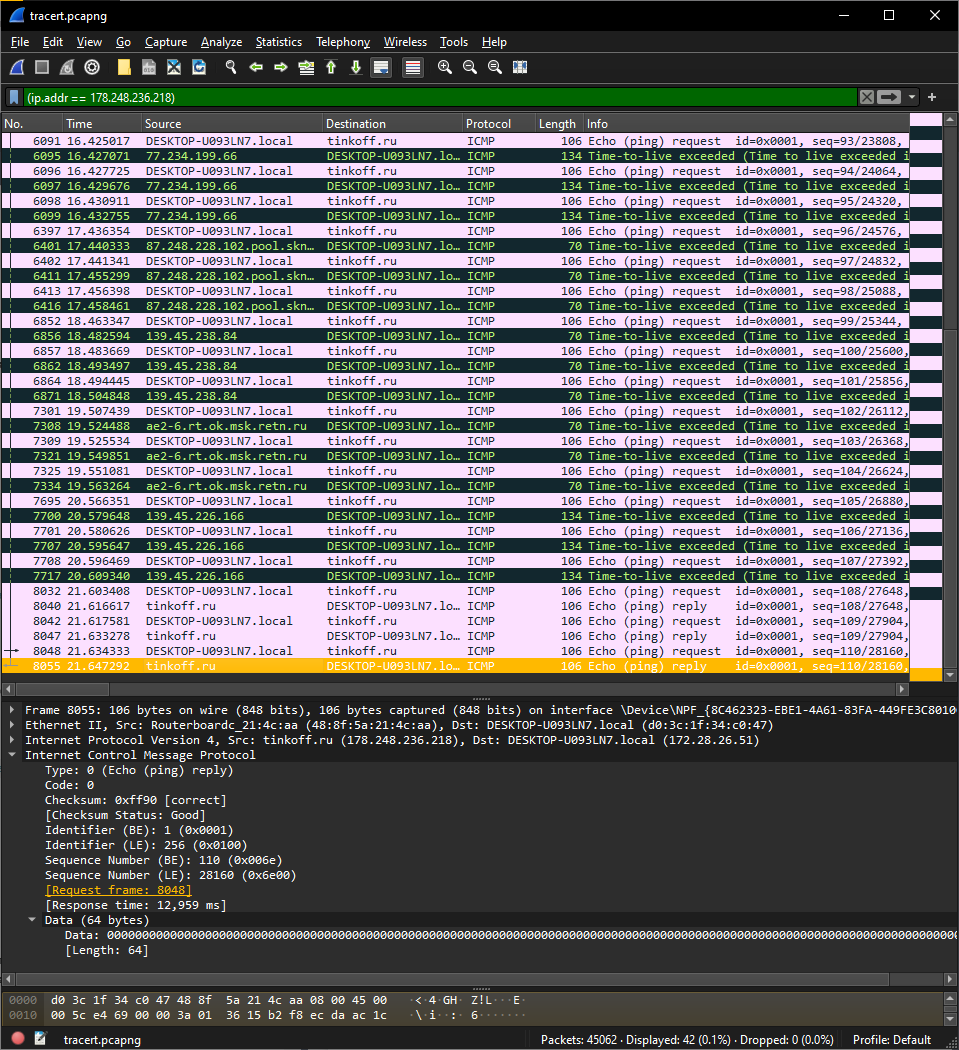
\includegraphics[width=1\linewidth]{res/tracert-wireshark.png}
    \caption{Tracert в Wireshark}
    \label{fig:tracert-wireshark}
\end{figure}

\begin{enumerate}
    \item Сколько байт содержится в заголовке IP? Сколько байт содержится в 
    поле данных? --- 20 + 64 байт
    \begin{figure}[H]
        \centering
        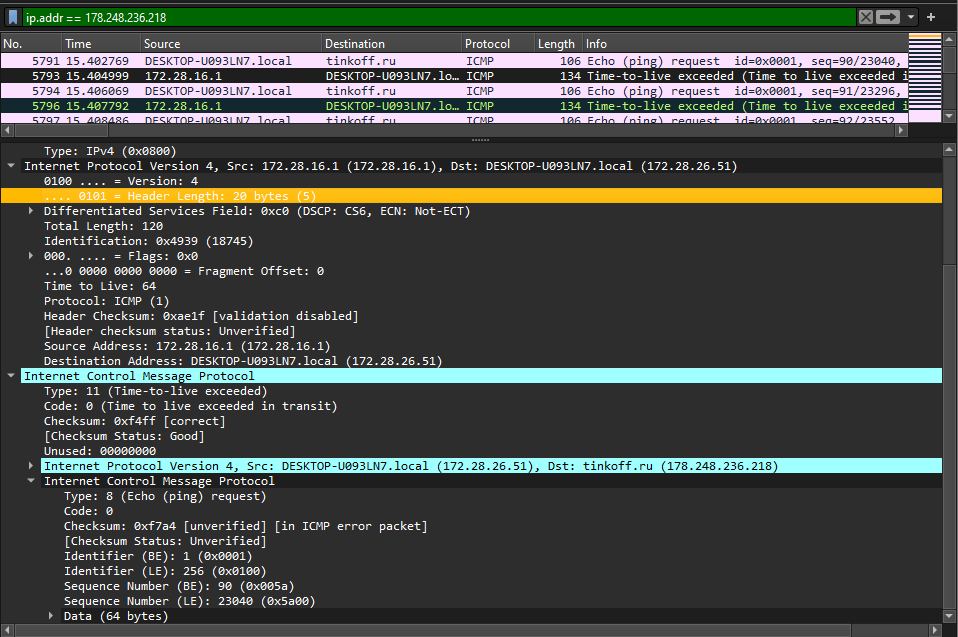
\includegraphics[width=1\linewidth]{res/tracert-data-size.png}
        \caption{Tracert data size}
        \label{fig:tracert-datasize}
    \end{figure}
    \item Как и почему изменяется поле TTL в следующих друг за другом ICMP пакетах tracert? Для ответа на этот вопрос нужно проследить изменение TTL при передаче по маршруту, состоящему из более чем двух хопов. --- Увеличивается на 1 каждый 3 пакет, для выявления расстояния в хопах.
    \begin{figure}[H]
        \centering
        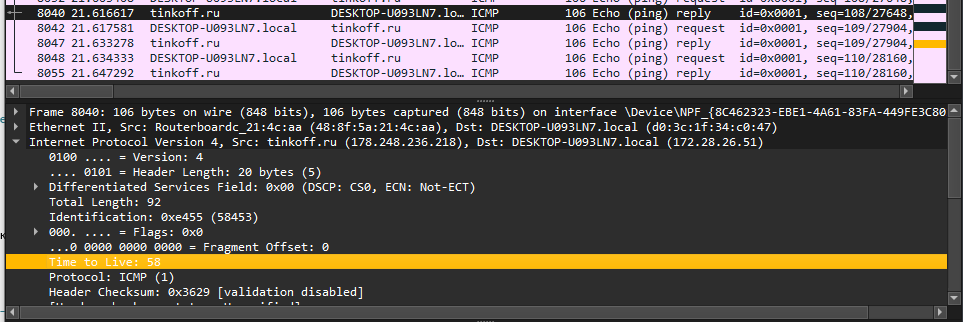
\includegraphics[width=1\linewidth]{res/tracert-ttl.png}
        \caption{Tracert TTL}
        \label{fig:tracert-ttl}
    \end{figure}
    \item Чем отличаются ICMP-пакеты, генерируемые утилитой tracert, от ICMP пакетов, генерируемых утилитой ping (см. предыдущее задание). --- В tracert происходит увеличение TTL
    \item Чем отличаются полученные пакеты «ICMP reply» от «ICMP error» и зачем нужны оба этих типа ответов? --- Различные значения в поле TYPE. ICMP reply: получение ответного сообщения; ICMP error: ошибка. 
    \item Что изменится в работе tracert, если убрать ключ «-d»? Какой 
    дополнительный трафик при этом будет генерироваться? --- ключ -d используется для того, чтобы предотвратить преобразование IP-адресов в имена хостов, eсли убрать ключ -d при использовании tracert, то утилита будет пытаться разрешать DNS-имена для каждого узла на пути
\end{enumerate}

\Subsection{Анализ HTTP-трафика}

Результат перехвата трафика в Wireshark: \ref{fig:http-wireshark}. Как можно видеть, HTTP-трафик скрывается за TLS, так что для просмотра заголовков GET-запроса нужно отслеживать сайт без TLS или каким-то образом добавить свои <<debug>>-сертификаты в Wireshark.

\begin{figure}[h]
    \centering
    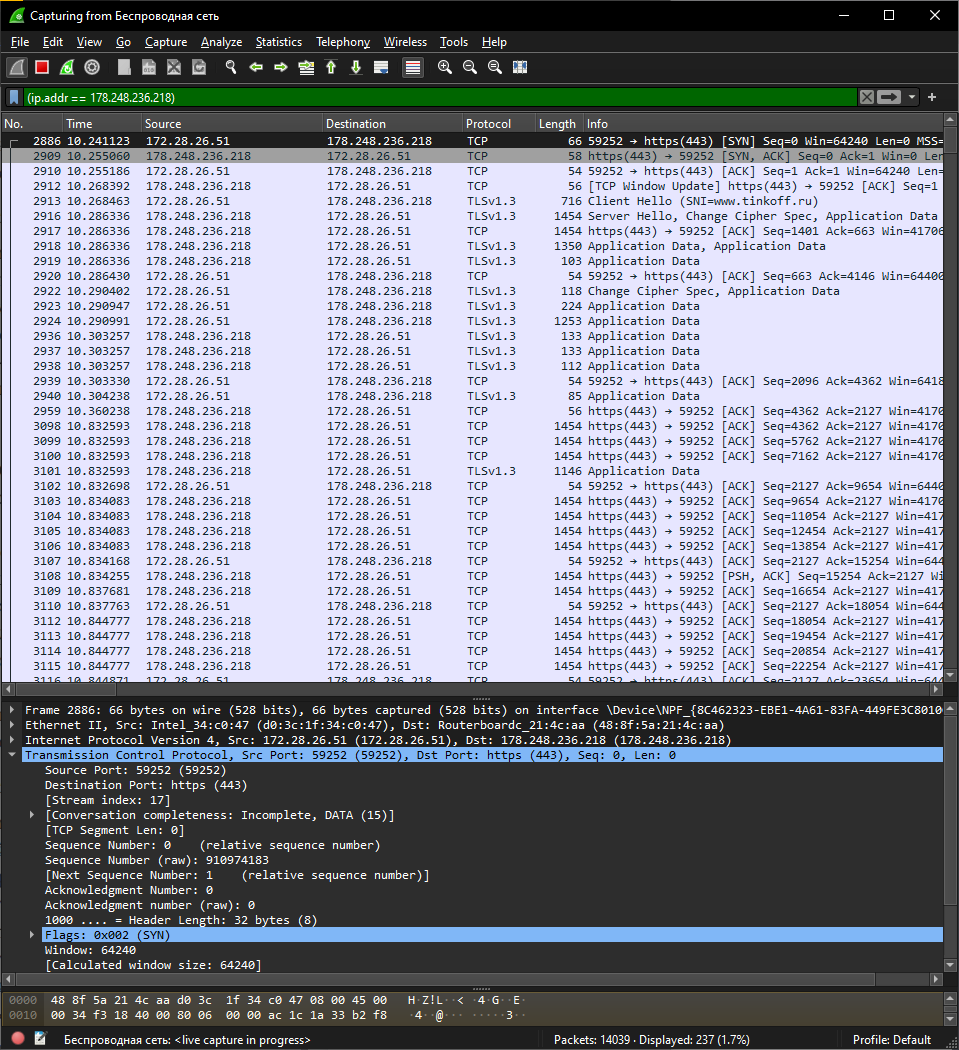
\includegraphics[width=1\linewidth]{res/http-wireshark.png}
    \caption{Http в Wireshark}
    \label{fig:http-wireshark}
\end{figure}

Для сайта без TLS результат будет примерно такой:

\begin{figure}[H]
    \centering
    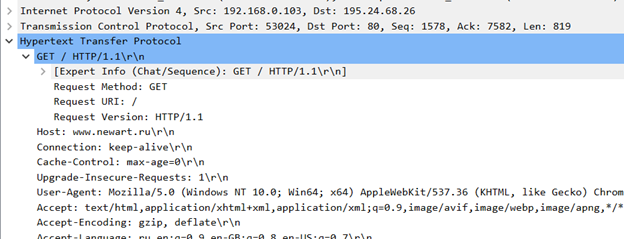
\includegraphics[width=1\linewidth]{res/http-no-tls.png}
\end{figure}

\begin{figure}[H]
    \centering
    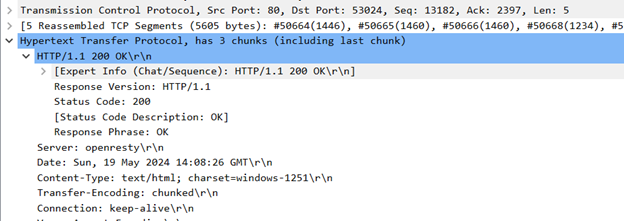
\includegraphics[width=1\linewidth]{res/http-no-tls-2.png}
\end{figure}

\Subsection{Анализ DNS-трафика}

Воспользуемся командой для сброса DNS-настроек в системе: \verb|ipconfig /flushdns|\;(рис. \ref{fig:dns-shell}).

\begin{figure}[h]
    \centering
    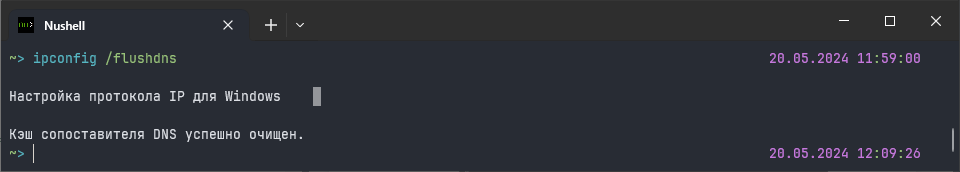
\includegraphics[width=1\linewidth]{res/dns-shell.png}
    \caption{Сброс настроек DNS}
    \label{fig:dns-shell}
\end{figure}

Результат перехвата трафика в Wireshrk в принципе совпадает с результатом предыдущего задания.

\begin{figure}
    \centering
    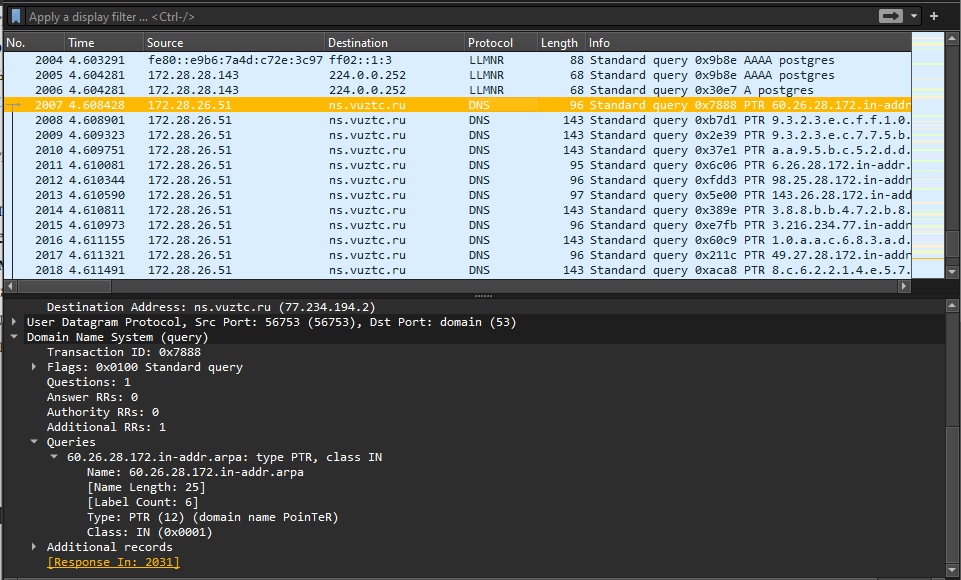
\includegraphics[width=1\linewidth]{res/dns-wireshark-no-filter.png}
    \caption{Перехват трафика DNS в Wireshark без фильтрации}
    \label{fig:dns-wireshark}
\end{figure}

\begin{enumerate}
    \item Почему адрес, на который отправлен DNS-запрос, не совпадает с 
адресом посещаемого сайта? --- Адрес отправки соответствует шлюзу по умолчанию, так как очищен кэш и нужно получить с DNS сервера адрес запрашиваемого сайта.
    \item Какие бывают типы DNS-запросов? --- \begin{itemize}
            \item \textit{Итеративный запрос} посылает доменное имя DNS-серверу и просит вернуть либо IP-адрес этого домена, либо имя DNS-сервера, авторитативного для этого домена. При этом сервер DNS не опрашивает другие серверы для получения ответа. 
            \item \textit{Рекурсивный запрос} посылает DNS-серверу доменное имя и просит возвратить IP-адрес запрошенного домена. При этом сервер может обращаться к другим DNS-серверам.
            \item \textit{Обратный запрос} посылает IP и просит вернуть доменное имя.
        \end{itemize}
    \item В какой ситуации нужно выполнять независимые DNS-запросы для 
получения содержащихся на сайте изображений? --- Когда картинки лежат на другом доменном имени.
\end{enumerate}

\Subsection{Анализ ARP-трафика}

Очистим таблицу ARP с помощью команды: \verb|netsh interface ip delete arpcache|\;, а проверим результат с помощью \verb|arp -a|\;. Результат очистки кажется неоднозначным, т.к. почти сразу там появляются новые записи, см. рис. \ref{fig:arp-shell}.

\begin{figure}[h]
    \centering
    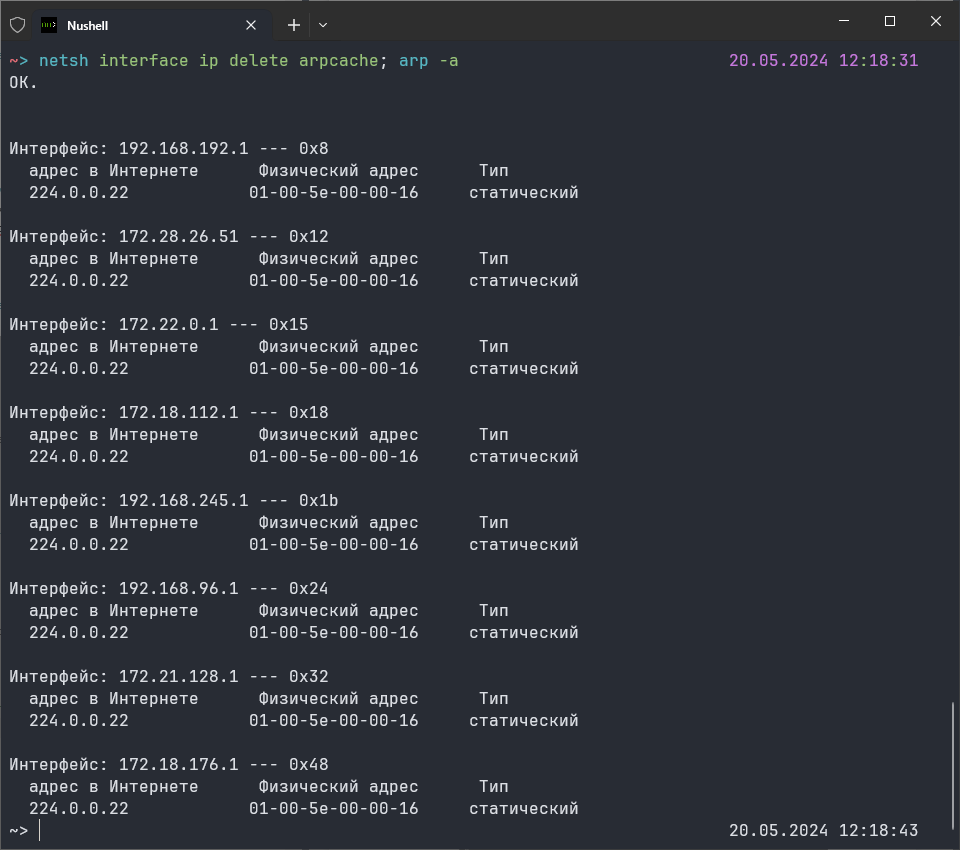
\includegraphics[width=1\linewidth]{arp-shell.png}
    \caption{Результат очистки ARP-таблицы}
    \label{fig:arp-shell}
\end{figure}

\begin{enumerate}
    \item Какие МАС-адреса присутствуют в захваченных пакетах ARP протокола? Что означают эти адреса? Какие устройства они идентифицируют? --- хостовой компьютер и мобильную точку доступа в телефоне.
        \begin{figure}[H]
            \centering
            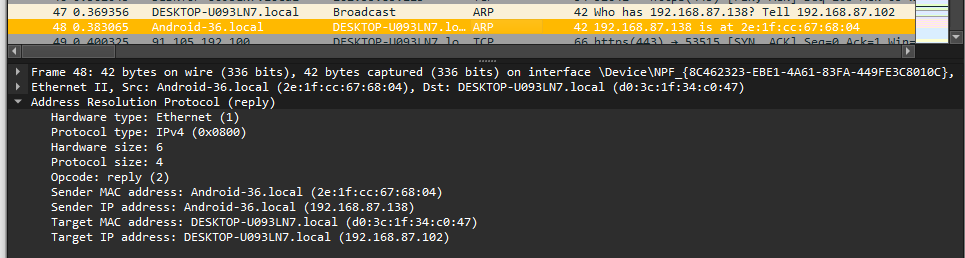
\includegraphics[width=1\linewidth]{res/arp-devices.png}
        \end{figure}
    \item Какие МАС-адреса присутствуют в захваченных HTTP-пакетах и что 
    означают эти адреса? Что означают эти адреса? Какие устройства они 
    идентифицируют? --- адрес отправляемого устройства, адрес принимающего устройства
    \begin{figure}[H]
        \centering
        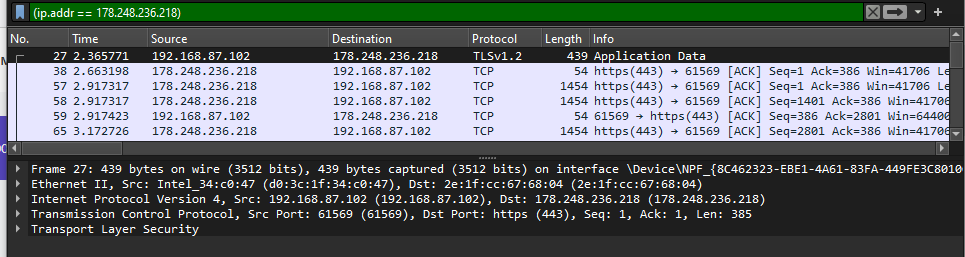
\includegraphics[width=1\linewidth]{res/arp-http-devices.png}
    \end{figure}
    \item Для чего ARP-запрос содержит IP-адрес источника? --- Что бы добавить информацию о узле в ARP таблицу
\end{enumerate}

\Subsection{Анализ трафика утилиты nslookup}

Выполним следующие команды: \verb|nslookup tinkoff.ru| и \verb|nslookup -type=NS tinkoff.ru|\;. Результат выполнения смотри на рис. \ref{fig:nslookup-shell}.

\begin{figure}[h]
    \centering
    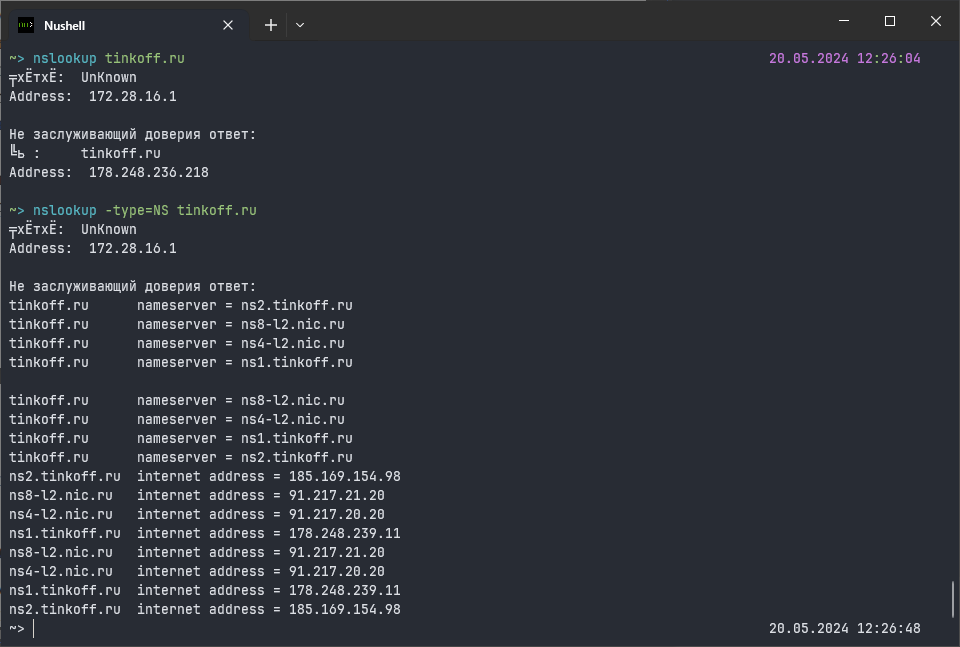
\includegraphics[width=1\linewidth]{res/nslookup-shell.png}
    \caption{Результат  выполнения Nslookup.}
    \label{fig:nslookup-shell}
\end{figure}

\begin{enumerate}
    \item Чем различается трасса трафика в п.2 и п.4, указанных выше? --- При запуске в п.2 утилита ищет IP-адрес хоста (запись типа A (IPv4) или AAAA (IPv6)).
    При запуске в п.4 утилита ищет Name Server для запрашиваемого хоста.
    \item Что содержится в поле «Answers» DNS-ответа? --- Данные запрашиваемого типа DNS-записи: для A - IPv4-адрес, для NS - список authoritative Name Server
    \item Каковы имена серверов, возвращающих авторитативный (authoritative) отклик? --- Авторитативный отклик возвращают серверы, которые являются ответственными 
    за зону, в которой описана информация, необходимая DNS-клиенту
\end{enumerate}

\Subsection{Анализ FTP-трафика}

Установим в Wireshrk фильтр \verb/ftp || ftp-data/\;. 

\begin{enumerate}
    \item Сколько байт данных содержится в пакете FTP-DATA? --- Размер может быть любы, но не больше MTU.
    \item Как выбирается порт транспортного уровня, который используется для 
передачи FTP-пакетов? --- Для потока управления на сервере используется порт 21. Для передачи данных используется порт 20, если передача идет в активном режиме, либо с любого 
порта клиента к любому порту сервера в пассивном режиме.
    \item Чем отличаются пакеты FTP от FTP-DATA? --- FTP используется для выполнения команд (request/response), а FTP-DATA работает с файлами.
\end{enumerate}

\Subsection{Анализ DHCP-трафика}

Установим в Wireshark фильтр \verb|bootp|. 

Выполним команды \verb|ipconfig /release| для сброса IP и \verb|ipconfig /renew| для обновления IP; результат см. на рис. \ref{fig:dhcp-shell-release} и рис. \ref{fig:dhcp-shell-renew}. Результат перехвата трафика в Wireshark можно видеть на рис. \ref{fig:dhcp-wireshark}.

\begin{figure}[h]
    \centering
    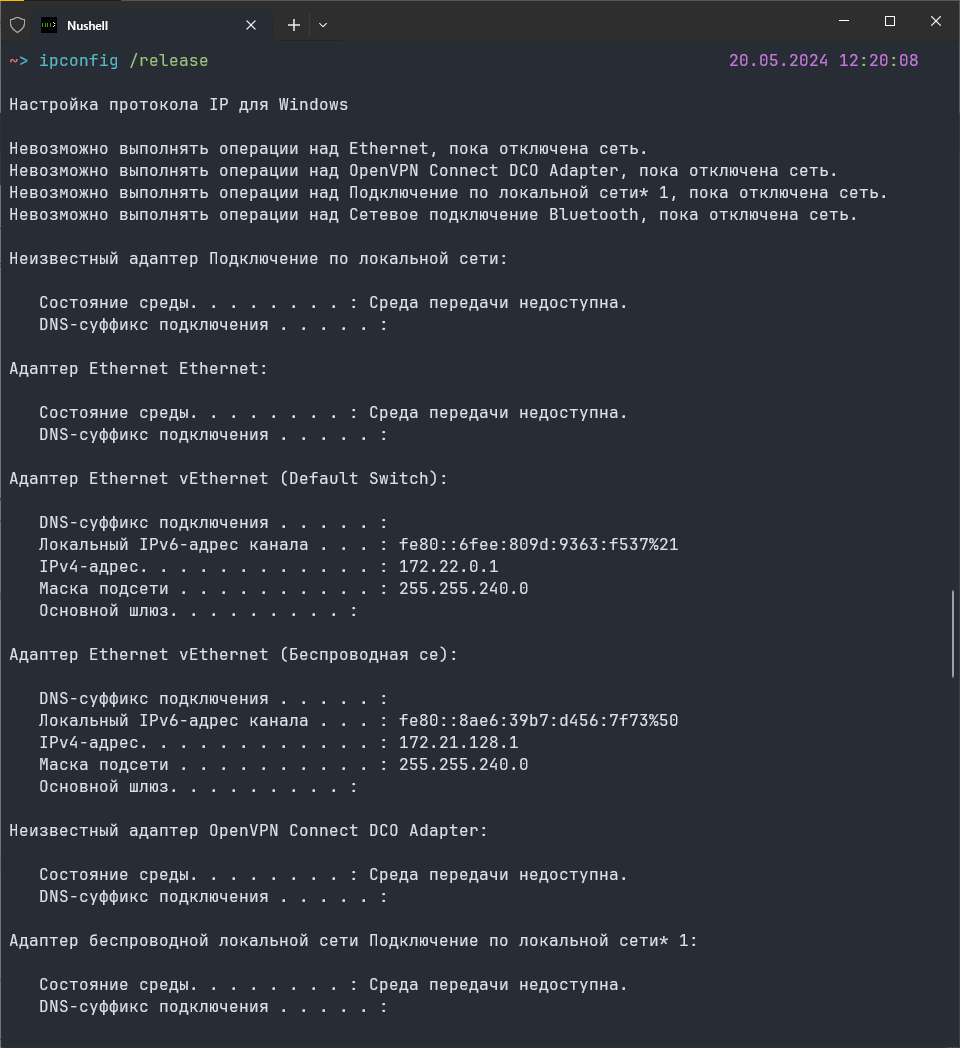
\includegraphics[width=1\linewidth]{res/dhcp-shell-release.png}
    \caption{Результат сброса IP}
    \label{fig:dhcp-shell-release}
\end{figure}

\begin{figure}[h]
    \centering
    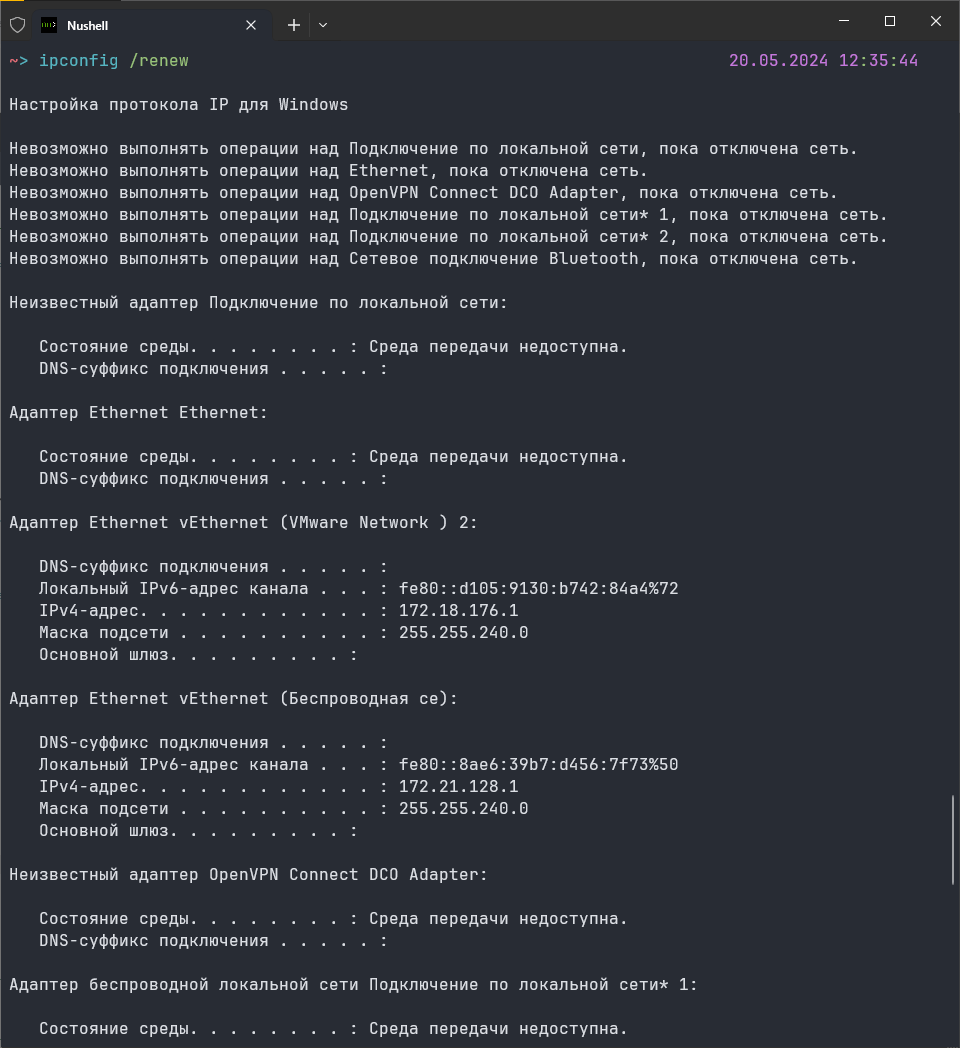
\includegraphics[width=1\linewidth]{res/dhcp-shell-renew.png}
    \caption{Результат обновления IP}
    \label{fig:dhcp-shell-renew}
\end{figure}

\begin{figure}
    \centering
    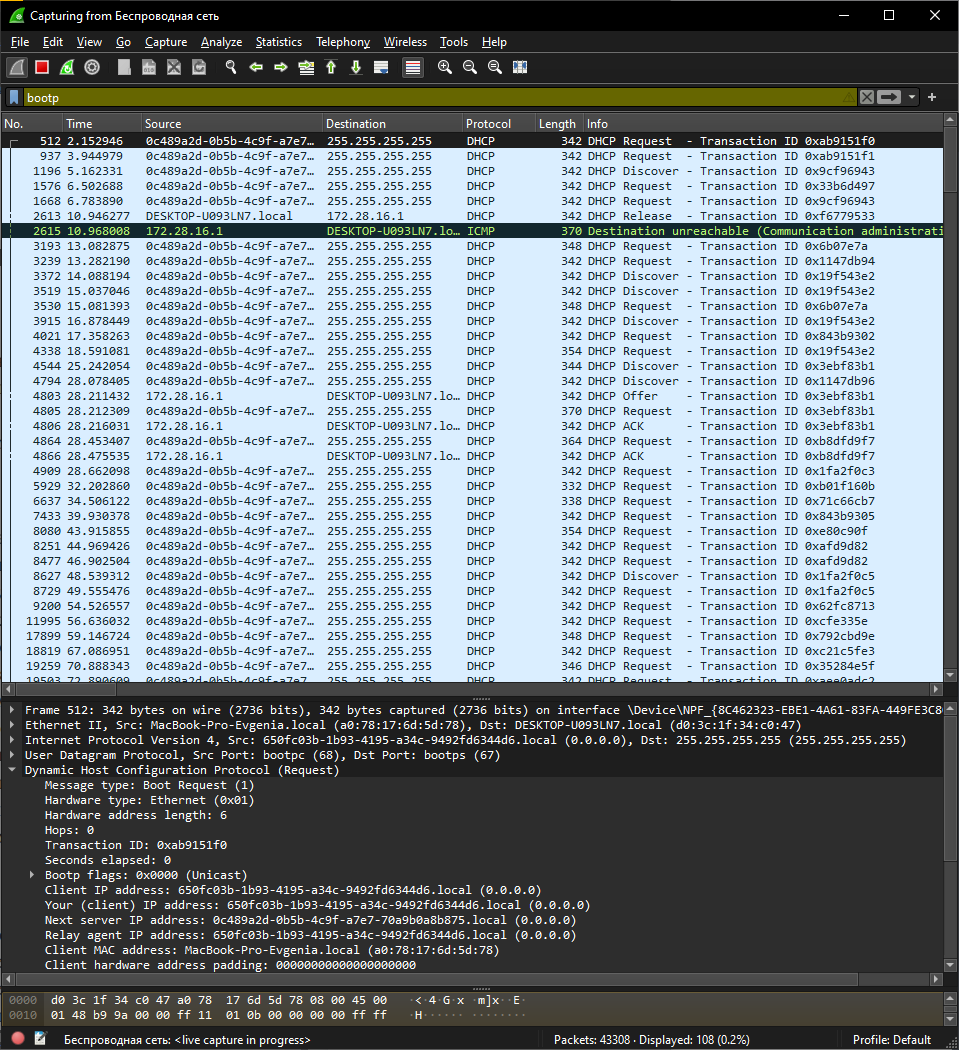
\includegraphics[width=1\linewidth]{res/dhcp-wireshark.png}
    \caption{Результат перехвата трафика в Wireshark при работе с DHCP}
    \label{fig:dhcp-wireshark}
\end{figure}

\begin{enumerate}
    \item Чем различаются пакеты «DHCP Discover» и «DHCP Request»? --- Оба запроса выполняются клиентом, DHCP Discover ищет DHCP-сервер в своей 
канальной среде, а DHCP Request принимает предлагаемый адрес и уведомляет 
DHCP-сервер об этом.
    \item Как и почему менялись MAC- и IP-адреса источника и назначения в 
    переданных DHCP-пакетах. --- В качестве MAC-адреса источника клиент изначально подставил свой MAC-адрес, а MAC-адрес сервера он не знает, поэтому использует широковещательный MAC адрес. Соответственно, в заголовке IP-пакета в качестве адреса источника клиент 
    использовал 0.0.0.0. При отправке Offer или ACK пакетов, адреса источника 
    соответствуют адресам DHCP-сервера, адреса назначения широковещательные.
    \item Каков IP-адрес DHCP-сервера? --- 172.128.16.1
    \begin{figure}[H]
        \centering
        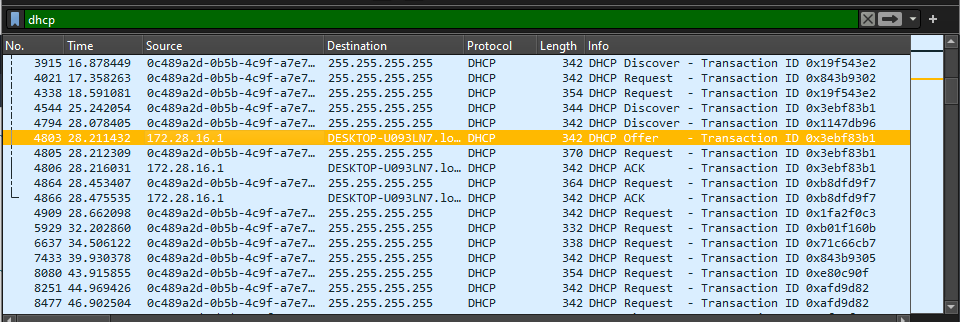
\includegraphics[width=1\linewidth]{res/dhcp-server-ip.png}
    \end{figure}
    \item Что произойдёт, если очистить использованный фильтр «bootp»? --- Будут отображаться все пакеты.
\end{enumerate}

\Subsection{Анализ Telegram-трафика}
\begin{itemize}
    \item Чем различаются пакета разных видов Telegram-трафика (текст, аудио, видео)? --- Текстовые данные передаются с помощью TSL. При загрузке аудио и видео используются TCP и SSLv2. Во время аудио-звонков используется TCP с SSL.
        \begin{figure}[H]
            \centering
            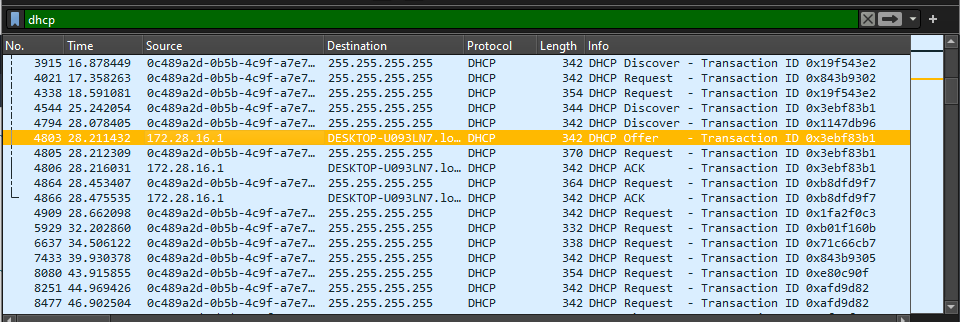
\includegraphics[width=1\linewidth]{res/telegram-wireshark.png}
        \end{figure}
    \item Какой Wireshark-фильтр следует использовать для независимой идентификации Telegram-трафика разных видов (текст, аудио, видео)?   
    --- В Wireshark можно установить фильтр по протоколу, соответственно нужно 
    установить \verb|tsl|, \verb|tcp|,  \verb|ssl|. При этом можно обнаружить, что весь трафик направляется на один (или несколько) IP адресов, поэтому можно еще фильтровать по нему, как я и сделал.
\end{itemize}

% \begin{figure}[H] % 'H' -- вставить тут же (подключен модуль), обычный вариант: 'htpb'
%     \centering
%     % { граница для иллюстрации
%     % \setlength{\fboxsep}{0pt}% убрать отсутп от границы
%     % \setlength{\fboxrule}{1pt}%
%     % \fbox{%
%             \includegraphics[width=\textwidth]{res/UML-class-diagram.png}
%     % }} % ограничение области действия параметров
%     \caption{Caption}
%     \label{fig:enter-label}
% \end{figure}

\Section{Вывод}

В ходе лабораторной работы был проанализирован сетевой трафик с помощью 
программы Wireshark. Изучили, какие пакеты передаются при работе утилит ping, и 
tracert и какую информацию они содержат. Также был проведен анализ трафика HTTP запросов и влияние на него кэширования данных. Кэширование также влияет на работу 
DNS, во время выполнения работы нам необходимо было очистить кэши и посмотреть на 
работу DNS-запросов. Далее был рассмотрен трафик при выполнении arp-запросов, для 
этого нужно было очистить arp-таблицу. Кроме того был проанализирован трафик при 
работе с FTP. И последним был рассмотрен трафик Telegram, мы узнали, какие протоколы 
используются в нем для передачи разных типов данных

%<<<<<<<<<<<<<<<<<<<<<< КОД РАБОТЫ <<<<<<<<<<<<<<<<<<<<<<<<


\end{document}
%<<<<<<<<<<<<<<<< ,,,,,,,,,,,,,,,,,,,,,,, <<<<<<<<<<<<<<<<<
%<<<<<<<<<<<<<<<<<<< СОДЕРЖИМОЕ ОТЧЕТА <<<<<<<<<<<<<<<<<<<<
